\documentclass[a4paper, 11pt]{report}
\usepackage{blindtext}
\usepackage[T1]{fontenc}
\usepackage[utf8]{inputenc}
\usepackage{titlesec}
\usepackage{fancyhdr}
\usepackage{geometry}
\usepackage{fix-cm}
\usepackage[hidelinks]{hyperref}
\usepackage{graphicx}
\usepackage{multirow}
\usepackage[english]{babel}
\usepackage{graphicx}
\usepackage{caption} 

\geometry{ margin=30mm }
\counterwithin{subsection}{section}
\renewcommand\thesection{\arabic{section}.}
\renewcommand\thesubsection{\thesection\arabic{subsection}.}
\usepackage{tocloft}
\renewcommand{\cftchapleader}{\cftdotfill{\cftdotsep}}
\renewcommand{\cftsecleader}{\cftdotfill{\cftdotsep}}
\setlength{\cftsecindent}{2.2em}
\setlength{\cftsubsecindent}{4.2em}
\setlength{\cftsecnumwidth}{2em}
\setlength{\cftsubsecnumwidth}{2.5em}


\begin{document}
\titleformat{\section}
{\normalfont\fontsize{15}{0}\bfseries}{\thesection}{1em}{}
\titlespacing{\section}{0cm}{0.5cm}{0.15cm}
\titleformat{\subsection}
{\normalfont\fontsize{13}{0}\bfseries}{\thesubsection}{0.5em}{}
\titlespacing{\section}{0cm}{0.5cm}{0.15cm}

%=======================================================================================

% #########################
% IMPORTANT - Add student names here!
% e.g. \newcommand{\stud1}{LOWE, David}
\newcommand{\studA}{{Fan Kaffa}}
\newcommand{\studB}{{Lin Link}}
\newcommand{\studC}{{Song Jared}}
\newcommand{\studD}{{Zheng Barnett}}
% ADD ANOTHER LINE FOR A FIFTH MEMBER
%
% IMPORTANT - Then give your SIDs
\newcommand{\sidA}{{510041359}}
\newcommand{\sidB}{{540801400}}
\newcommand{\sidC}{{550155230}}
\newcommand{\sidD}{{550718806}}
% ADD ANOTHER LINE FOR A FIFTH MEMBER

%
% IMPORTANT - And then update which major each student will focus on
\newcommand{\majA}{{Computer Science}}
\newcommand{\majB}{{Data Science}}
\newcommand{\majC}{{SW Development}}
\newcommand{\majD}{{Cyber Security}}
% ADD ANOTHER LINE FOR A FIFTH MEMBER - HCI

% #########################


\pagenumbering{Alph}
\begin{titlepage}
\begin{flushright}

\includegraphics[width=4cm]{USyd}\\[1cm] 
\end{flushright}

\begin{centering}
\textbf{\huge INFO1111: Computing 1A Professionalism}\\[0.75cm]
\textbf{\huge 2025 Semester 1}\\[2cm]
\textbf{\huge Skills: Team Project Report}\\[2cm]

\textbf{\large Submission number: T4 SL Group 6 (1)}\\[0.5cm]
{\large \textbf{Github link: \url{https://github.com/KaltsitFan/INFO1111_GROUP.git}}}\\[0.75cm]
\textbf{\huge Team Members:}\\[0.75cm]

\begin{tabular}{|p{0.25\textwidth}|p{0.13\textwidth}|p{0.12\textwidth}|p{0.12\textwidth}|p{0.22\textwidth}|}
	\hline
	\multirow{2}{*}{Name} & \multirow{2}{*}{Student ID} & Target * & Target * & \multirow{2}{*}{Selected Major} \\
	 & & Foundation & Advanced & \\
	\hline
	\hline
	\raggedright{\studA} & \sidA & AG & NA & Computer Science \\
	\hline
	\raggedright{\studB} & \sidB & A & NA & \majB \\
	\hline
	\raggedright{\studC} & \sidC & A & NA & \majC \\
	\hline
	\raggedright{\studD} & \sidD & A & NA & \majD \\
	\hline
\end{tabular}
\\[0.5cm]
\end{centering}

* Use the following codes:
\begin{itemize}
\setlength\itemsep{0em}
\item NA = Not attempting in this submission
\item A = Attempting (not previously attempting)
\item AW = Attempting (achieved weak in a previous submission) 
\item AG = Attempting (achieved good in a previous submission)
\item S = Already achieved strong in a previous submission
\end{itemize}

\thispagestyle{empty}
\end{titlepage}
\pagenumbering{arabic}


%=======================================================================================

\tableofcontents

%=======================================================================================
\newpage

\section{Group Response}

Our team, composed of members from different computing majors, effectively utilized GitHub's issue tracker for task allocation, enabling clear responsibility assignments and progress tracking. Cross-disciplinary collaboration played a crucial role—our Software Development member assisted the Cybersecurity member in coding challenges, while our Data Science member guided data-related tasks. Initially, LaTeX documentation presented significant challenges due to frequent syntax errors and lack of real-time previews. Transitioning to Visual Studio Code with LaTeX extensions resolved these issues by enabling immediate error detection and correction. Through structured GitHub management and mutual technical support, our collaborative approach markedly improved communication, efficiency, and overall project management effectiveness.


\newpage
\section{Individual Response}

\subsection{Skills for Computer Science: Kaffa Fan }
In the disaster response system project, my primary responsibilities included the establishment of the overall system architecture, the setup of the GitHub collaboration framework, and the configuration of the LaTeX documentation environment. Reflecting based on the SFIA framework, I selected the following two skills:

\textbf{Software Development (PROG)}

According to the SFIA framework~\cite{sfia}, software development is foundational to implementing technological solutions. For the LA wildfire disaster response scenario, effectively managing documentation using LaTeX was critical to ensure rapid generation and dissemination of accurate reports. Initially, our team frequently encountered LaTeX syntax errors such as missing commands missing commands (\textbackslash end{itemize})
 due to using editors without real-time preview capabilities. By transitioning to Visual Studio Code with LaTeX extensions, we could immediately identify and rectify these errors, significantly reducing documentation delays. This directly supported emergency response requirements, enabling quick delivery of clear instructions and updates to responders. Additionally, my demonstrated ability to compile and manage documents via the Git terminal further ensured smooth, efficient project documentation workflows.

\textbf{Skill Enhancement (Team Collaboration Details):}  
Introducing real-time preview tools considerably enhanced the team's productivity and accuracy, minimizing errors and speeding up response times—key factors during an emergency.

\textbf{Areas for Further Improvement:}  
Despite improvements, I identified an over-reliance on tool-based error detection. In future projects, I aim to improve my manual code review skills, ensuring reliability even when technological resources are limited, a critical capability in disaster situations.

\textbf{Systems Integration and Build (SINT)}

According to the SFIA framework~\cite{sfia}, effective systems integration is essential for creating a coherent and responsive disaster management system. In the context of the wildfire scenario, my role involved integrating various system components, such as real-time data interfaces and a user-friendly incident dashboard for emergency personnel. Early in the project, unclear task assignments created confusion among team members. Implementing GitHub Issues significantly clarified roles and responsibilities, specifically tasks like "Frontend Interface (Incident Dashboard)" and "Data Interface Development (Real-time Sensor Feeds)," streamlining integration processes. My consistent use of Git for task management and module synchronization (Figures 4) ensured efficient module integration, crucial for rapid deployment in emergency scenarios.

\textbf{Skill Enhancement (Team Collaboration Details):}  
Clear task definition through GitHub substantially improved our integration capability, facilitating quick and smooth development of crucial disaster-response features, such as real-time dashboards.

\textbf{Areas for Further Improvement:}  
Our technical discussions sometimes involved excessive jargon, complicating interdisciplinary communication. Moving forward, simplifying complex technical concepts into clear, accessible language will be essential, particularly in high-stakes, collaborative disaster-response environments.


\newpage

\section*{3. Git Response}

\textbf{1. Clone the repository}

Clone the remote repository to your local computer:
\begin{verbatim}
git clone https://github.com/KaltsitFan/INFO1111_T4_SL_GROUP_6
\end{verbatim}

This picture illustrates the cloning process: 

\begin{center}
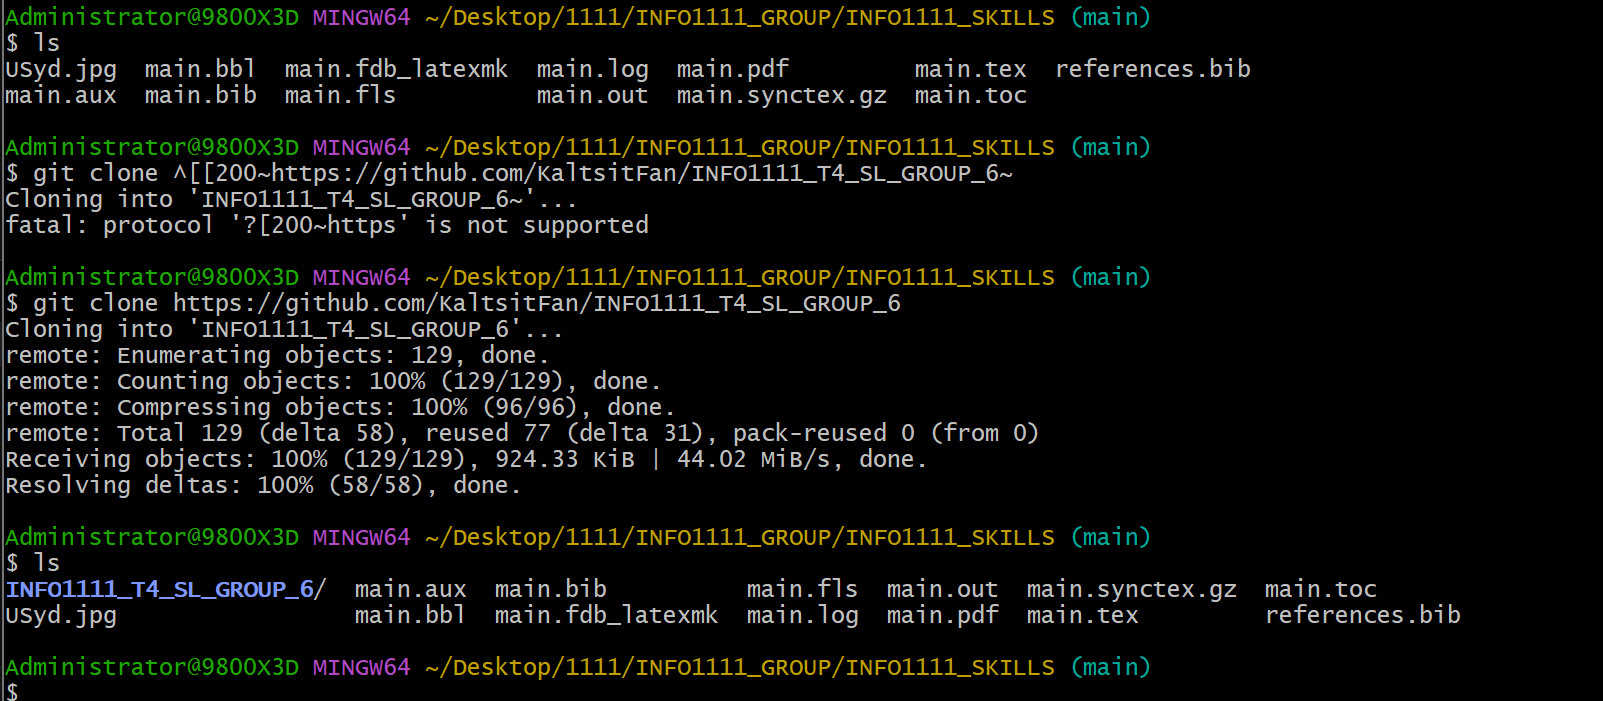
\includegraphics[width=0.8\textwidth]{kaffa/clone.png}
\captionof{figure}{Cloning the repository}
\end{center}

\textbf{2. Stage, Commit, Push, and Check Status}

Stage all modified files, commit the changes with a clear message, push the committed changes to GitHub, and verify the repository status:

\begin{verbatim}
git add .
git commit -m "Your commit message"
git push
git status
\end{verbatim}

This picture demonstrates staging, committing, pushing, and checking status:

\begin{center}
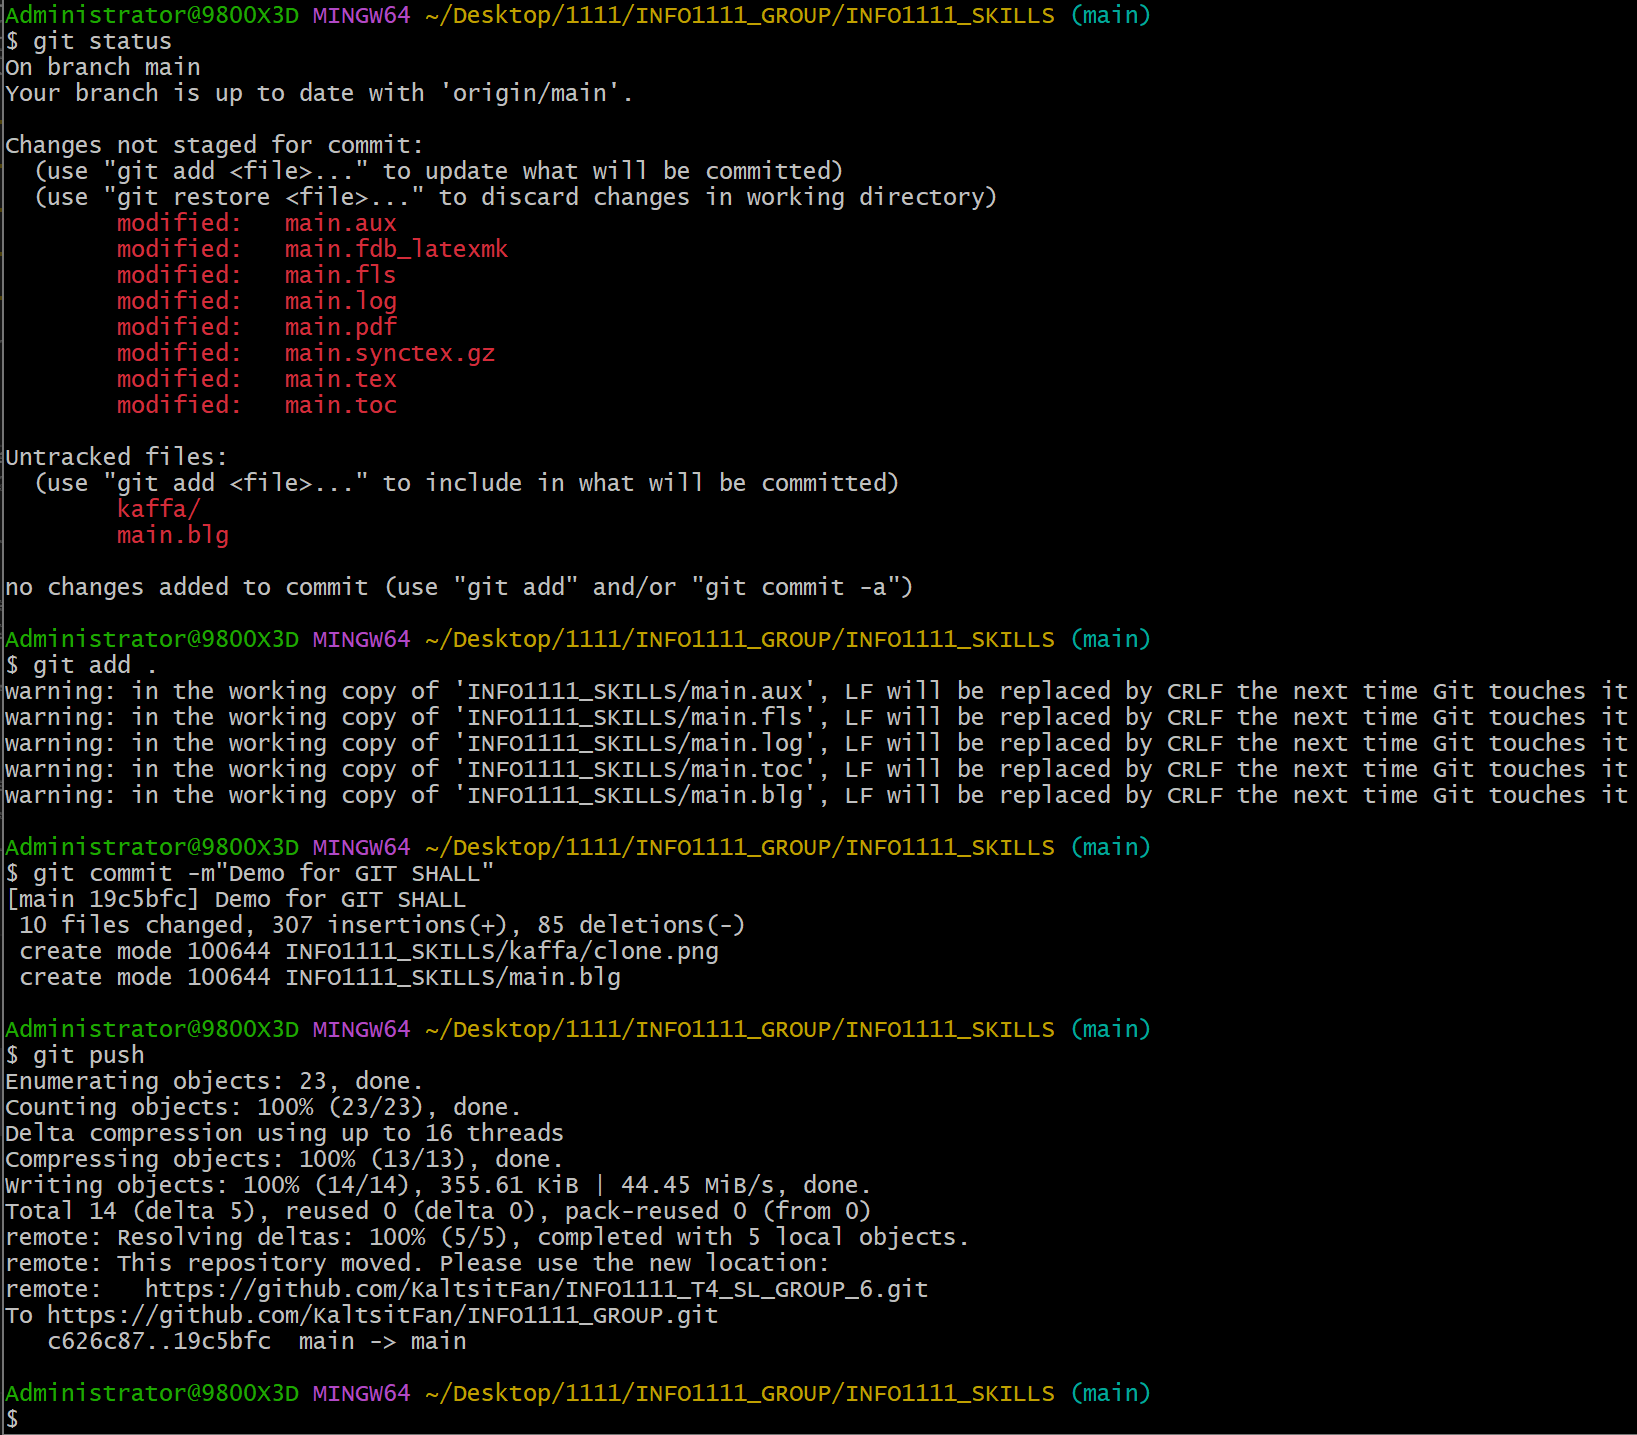
\includegraphics[width=0.8\textwidth]{kaffa/push.png}
\captionof{figure}{Staging, committing, pushing changes, and checking status}
\end{center}

\textbf{3. Synchronize with remote repository}

Pull the latest updates from the GitHub repository to synchronize your local repository:

\begin{verbatim}
git pull origin main
\end{verbatim}

This picture shows synchronizing the local repository with remote updates:

\begin{center}
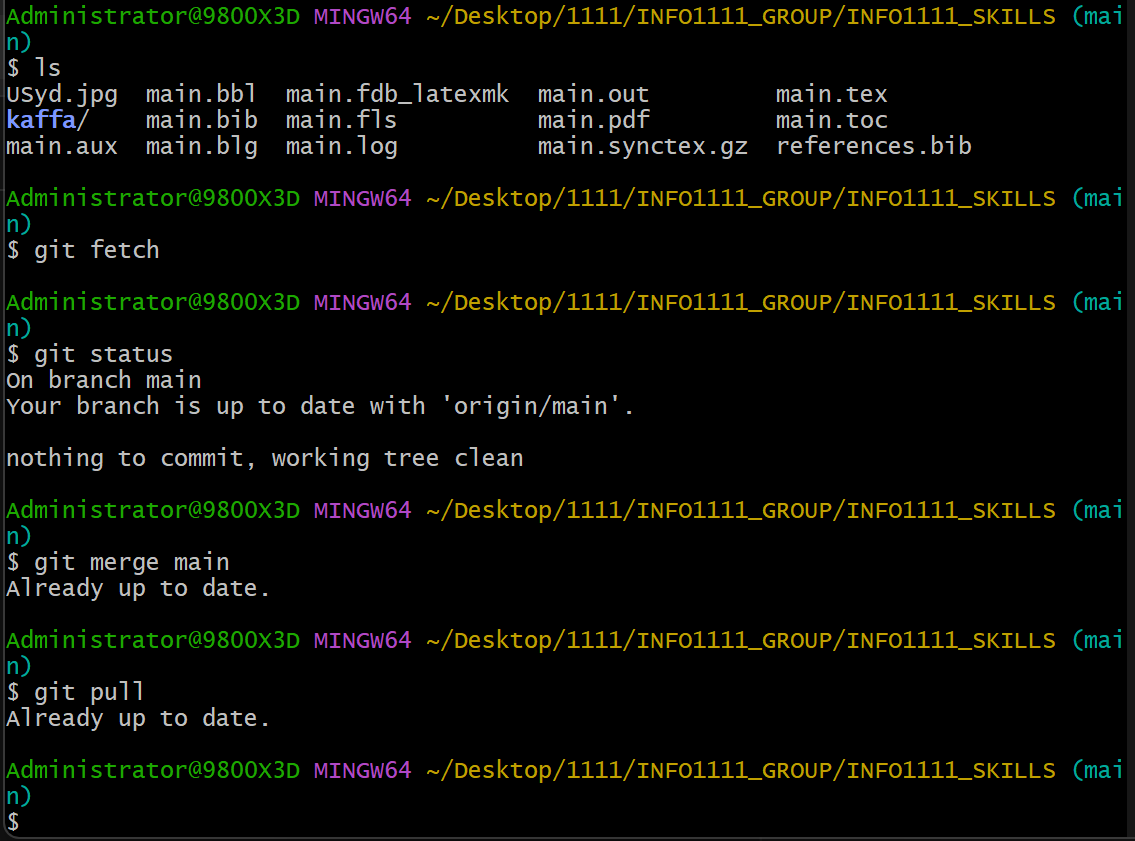
\includegraphics[width=0.8\textwidth]{kaffa/synchronize.png}
\captionof{figure}{Pulling latest changes from remote repository}
\end{center}


\textbf{4. Generate PDF using Git Terminal}

Compile your LaTeX document into PDF using Git terminal commands:

\begin{verbatim}
bibtex main.aux and pdflatex yourfile.tex
\end{verbatim}

This generates a PDF document from your LaTeX file directly via terminal. Bibtex make sure citation correct

This picture illustrates generating a PDF using terminal:

\begin{center}
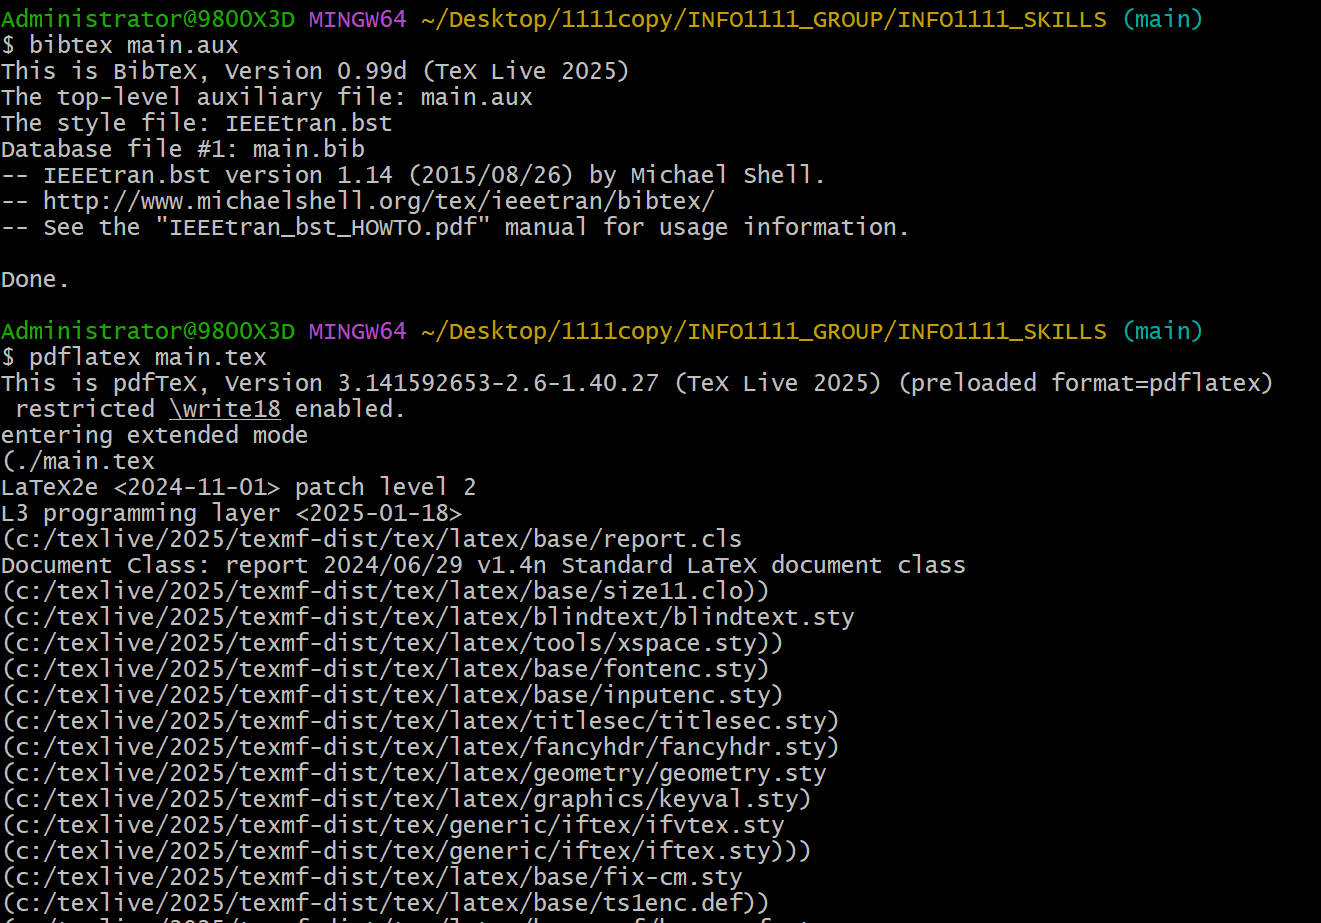
\includegraphics[width=0.8\textwidth]{kaffa/forpdf.png}
\end{center}






\newpage

\subsection{Skills for SW Development: Jared Song}
Through this project, I identified two critical skills from the SFIA framework relevant to software development:

\subsubsection{Key Technical Skills}
\begin{itemize}
    \item \textbf{PROG (Programming/Software Development)} \\
    According to the SFIA framework~\cite{sfia}, developing the disaster system's offline functionality required:
    \begin{itemize}
        \item Implementing local data caching using Python's \texttt{shelve} module
        \item Writing thread-safe code for concurrent access during emergencies
    \end{itemize}

    \item \textbf{TEST (Software Testing)} \\
    Establish comprehensive test coverage for disaster scenarios:
    \begin{itemize}
        \item Parameterized test suite covering distinct failure modes:
        \begin{itemize}
            \item Network partitions (simulated with \texttt{pytest-timeout})
            \item Data corruption (CRC32 validation tests)
            \item Resource exhaustion (memory/stress tests)
        \end{itemize}

        \item Mock service framework featuring:
        \begin{itemize}
            \item Configurable failure injection 
            \item Latency simulation 
            \item Stateful behavior modeling
        \end{itemize}
    \end{itemize}
\end{itemize}

\subsubsection{Skill Development through Collaboration}
According to the SFIA framework~\cite{sfia}, The team environment enhanced these skills by:
\begin{itemize}
    \item \textbf{Cross-domain feedback}: Data Science members' statistical analysis helped refine our cache invalidation algorithm, the data collected has also simplified the work and made the work more straightforward.
    \item \textbf{Collective problem-solving}: Pair programming sessions fixed race conditions in the resource allocator module
    \item \textbf{Tool knowledge sharing}: Learned GitHub Actions CI configuration from Computer Science teammate, which really helps me enhance my skills and understanding of GitHub.
\end{itemize}

\subsubsection{Areas for Improvement}  
Through my work on the disaster response system, I've identified several technical and professional skills that require refinement: 
\begin{itemize}
    \item \textbf{Performance Optimization}: Need deeper understanding of profiling tools (e.g. cProfile) - evidenced when our stress tests failed at 10,000+ concurrent users, be able to learn more about Python and be proficient in using Python. 
    \item \textbf{Technical Documentation}: Find difficulty in using Github and Latex, so learning more skills and implementing automated documentation generation are important.
\end{itemize}

\newpage

\subsection*{Git Response}

\textbf{1. Clone the repository}

Clone the remote repository to local computer:
\begin{center}
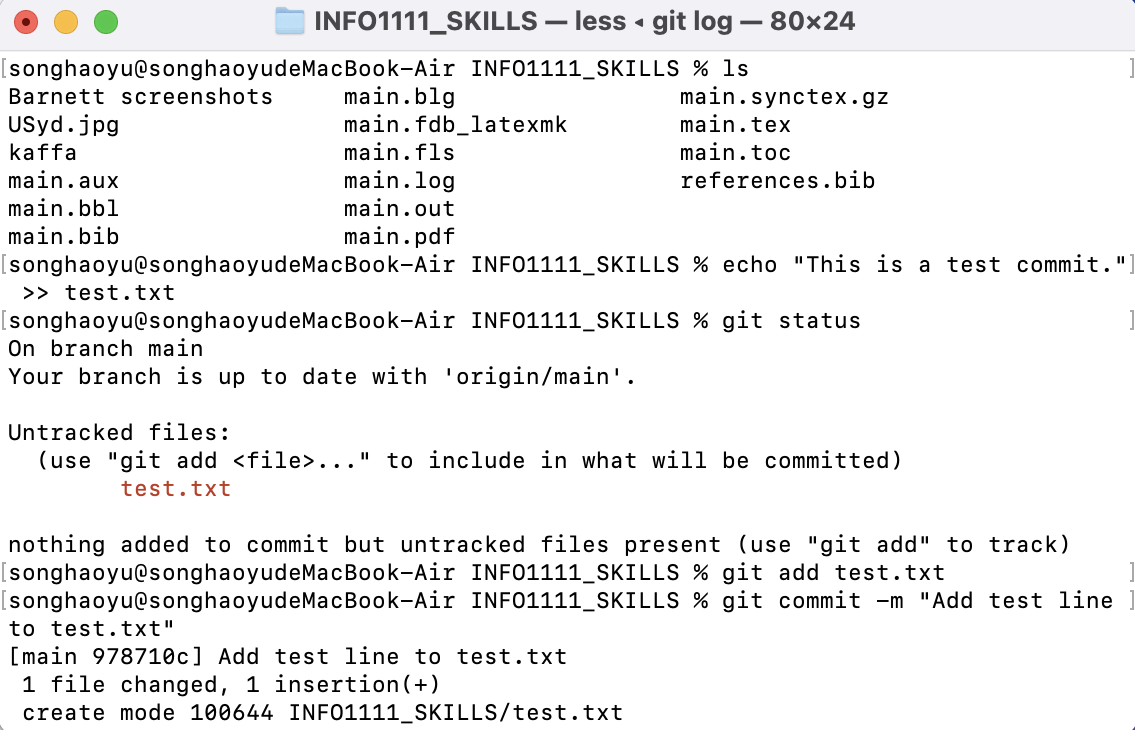
\includegraphics[width=0.8\textwidth]{Jared/clone.png}
\captionof{figure}{Cloning the repository}
\end{center}

\textbf{2. Commit and push changes to local repository}
\begin{center}
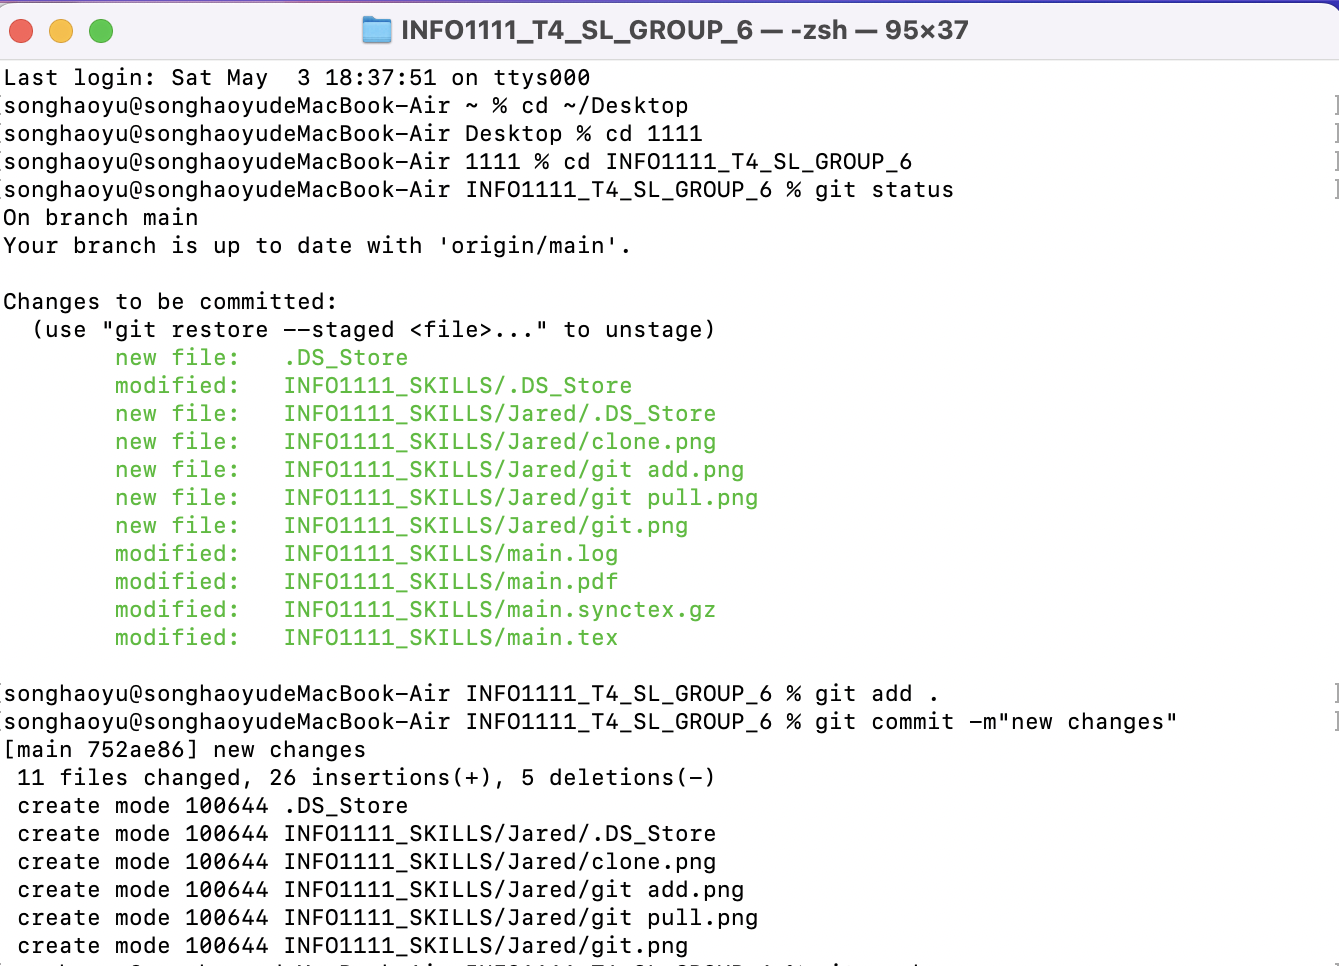
\includegraphics[width=0.8\textwidth]{Jared/gitadd.png}
\end{center}
\begin{center}
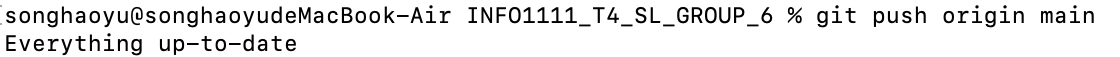
\includegraphics[width=0.8\textwidth]{Jared/gitpush.png}  
\end{center}

\textbf{3. Synchronize repository}
\begin{center}
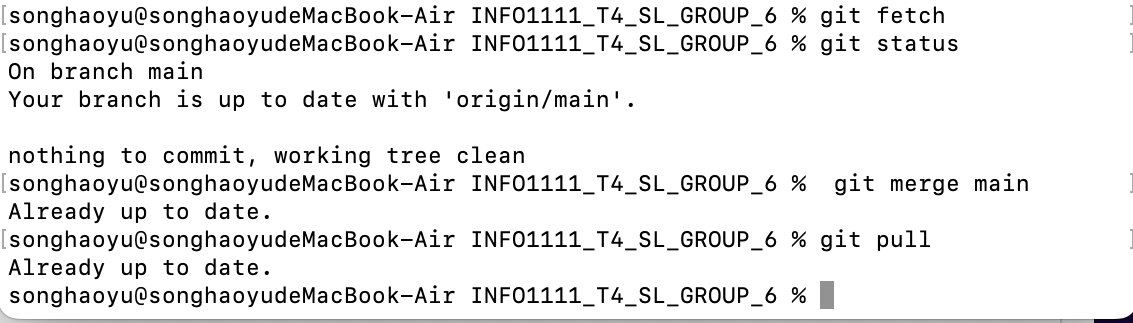
\includegraphics[width=0.8\textwidth]{Jared/git pull.png}  
\captionof{figure}{Pulling latest changes from remote repository}
\end{center}

\textbf{4. PDF Generation Through Git CLI}
\begin{center}
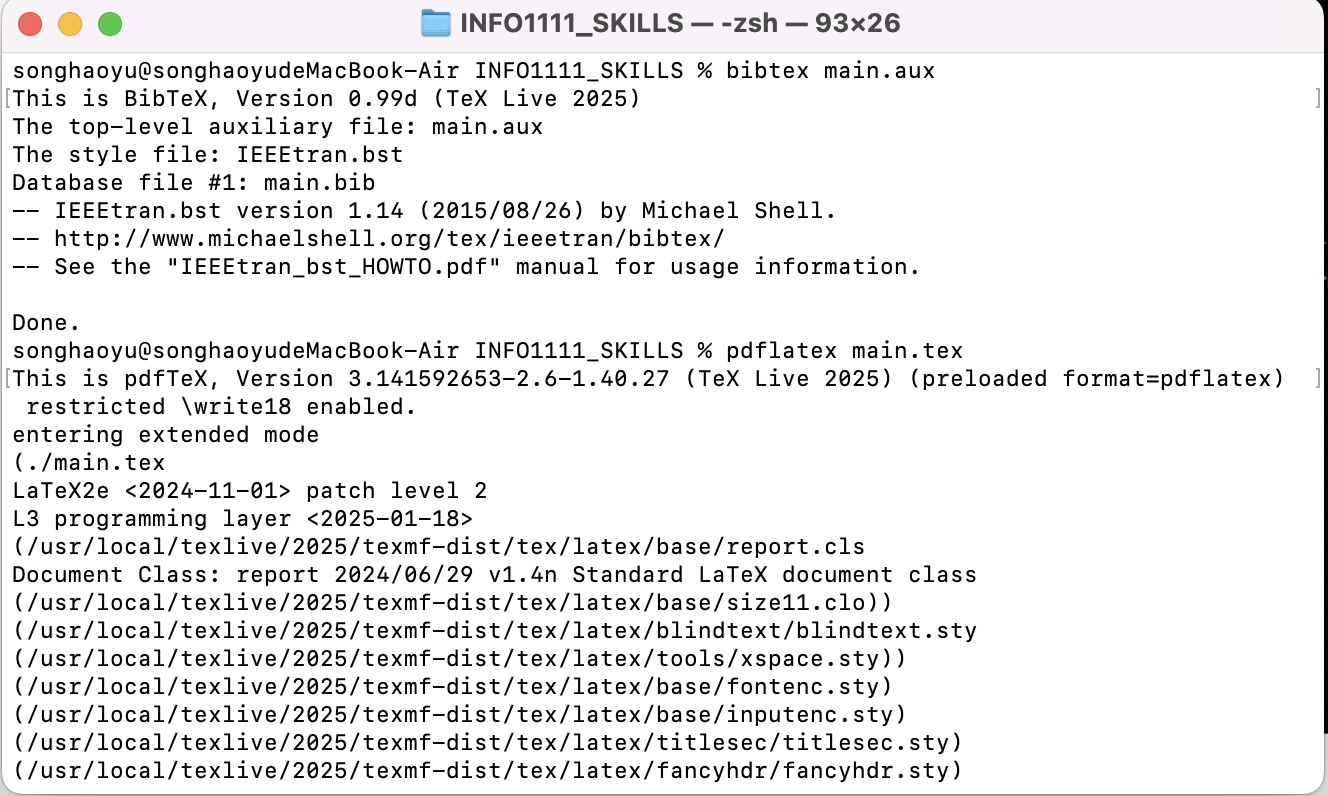
\includegraphics[width=0.8\textwidth]{Jared/git.png}  
\end{center}


\newpage

\subsection{Skills for Cybersecurity: Barnett Zheng}
Through this project, I identified two critical skills from the SFIA framework relevant to cybersecurity:

\subsubsection{Key Technical Skills}
\begin{itemize}
    \item \textbf{SCTY (Network Security)}~\cite{network_security} \\
    Securing communication channels in the disaster response system required:
    \begin{itemize}
        \item Implementing firewall rules to restrict unauthorized access
        \item Encrypting data transmissions using TLS to ensure confidentiality
        \item Deploying intrusion detection systems (IDS) to monitor for suspicious activity
    \end{itemize}

    \item \textbf{SCTY (Data Protection)}~\cite{data_protection} \\
    Ensuring the privacy and integrity of user data involved:
    \begin{itemize}
        \item Utilizing AES encryption for sensitive personal information storage
        \item Implementing access controls to restrict unauthorized data retrieval
        \item Performing regular security audits to detect vulnerabilities
    \end{itemize}
\end{itemize}

\subsubsection{Skill Development through Collaboration}
The team environment enhanced these cybersecurity skills by:
\begin{itemize}
    \item \textbf{Interdisciplinary Insights}: Working with software engineers helped me align security mechanisms with application logic, ensuring seamless integration.
    \item \textbf{Incident Response Drills}: Collaborating with the team in security simulations improved my ability to detect and mitigate threats quickly.
    \item \textbf{Knowledge Sharing}: Gained practical experience with GitHub security features, such as dependency scanning and secret detection.
\end{itemize}

\subsubsection{Areas for Improvement}  
Through my work on the disaster response system, I've identified several cybersecurity skills that require further refinement:
\begin{itemize}
    \item \textbf{USUP (Incident Response)}~\cite{incident_response}: Need to enhance my ability to analyze and react to security breaches in real time, particularly in high-pressure situations.
    \item \textbf{RESL (Risk Assessment)}~\cite{risk_assessment}: Improve my ability to evaluate and prioritize security threats, ensuring that mitigation efforts focus on the most critical risks.
\end{itemize}  

\newpage

\section*{2.3.1. Git Response}

\textbf{1. Clone the repository}

Clone the remote repository to your local computer:

\begin{center}
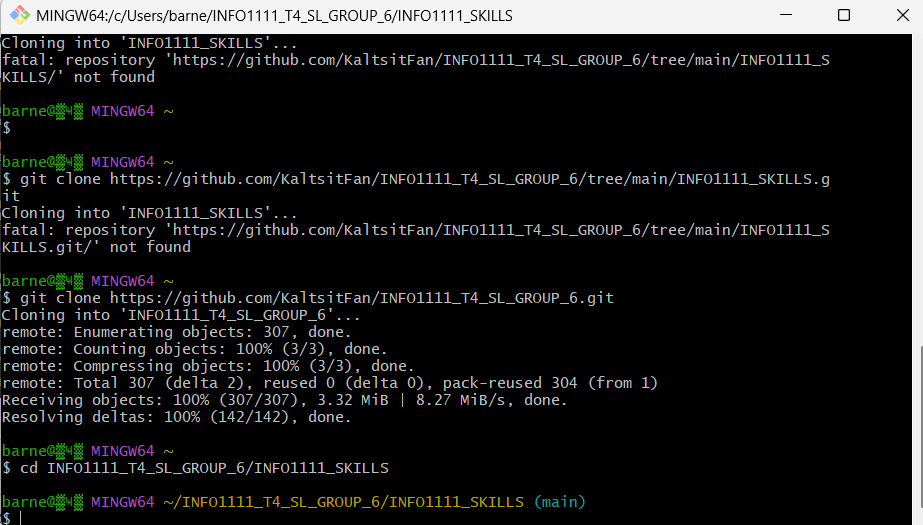
\includegraphics[width=0.8\textwidth]{BZ/1.png}
\captionof{figure}{Cloning the remote repository}
\end{center}

\subsection*{2. Standard Development Cycle}
The regular workflow for making changes consists of these steps:
\begin{verbatim}
git add .                          # Stage all modified files
git commit -m "Descriptive message" # Commit changes locally
git status                         # Verify repository state
\end{verbatim}

\begin{center}
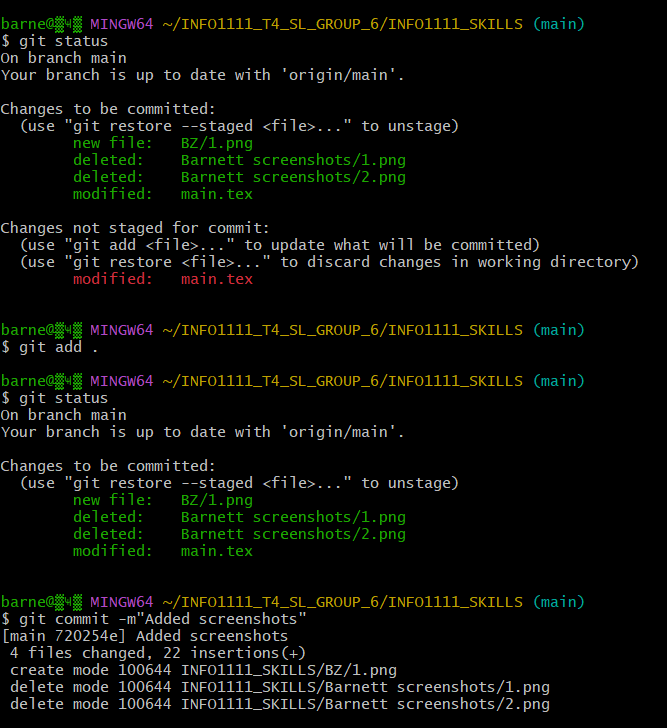
\includegraphics[width=0.8\textwidth]{BZ/2.png}
\captionof{figure}{Git workflow: staging, committing}
\end{center}

\subsection*{3. Document Compilation}
Generate the project PDF through terminal commands:
\begin{verbatim}
pushing oringin main
bibtex main.aux      # Process citations
pdflatex main.tex    # Final compilation
\end{verbatim}

\begin{center}
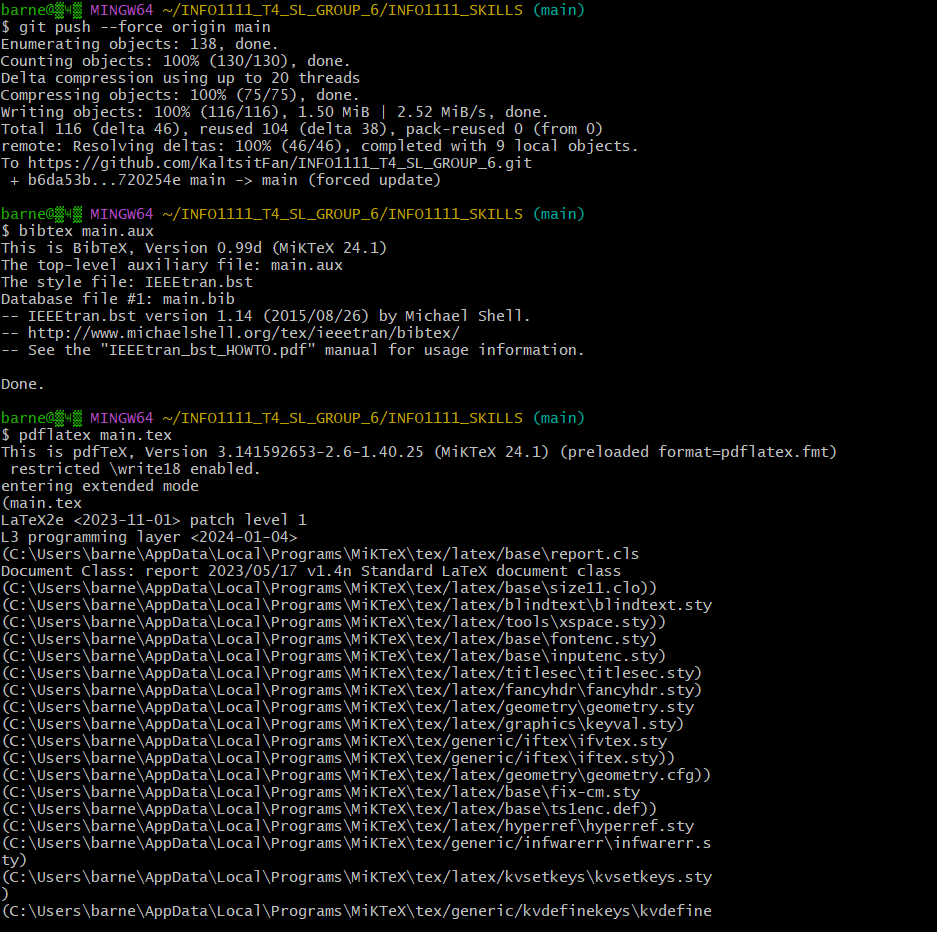
\includegraphics[width=0.8\textwidth]{BZ/3.png}
\captionof{figure}{Compiling LaTeX document to PDF and pushing}
\end{center}

\subsection*{Skills for Data Science: Link Lin}

Through my work exploring data science applications, particularly in disaster response and predictive analytics, I identified two critical skills relevant to data science based on their practical importance:

\subsubsection*{Key Technical Skills}
\begin{itemize}
    \item \textbf{Data Integration} \\
    Effective data integration for disaster scenarios required:
    \begin{itemize}
        \item Combining diverse datasets (e.g., satellite imagery, weather forecasts) using Python’s \texttt{Pandas} library
        \item Normalizing inconsistent formats for real-time visualization during emergencies
    \end{itemize}

    \item \textbf{Predictive Modeling} \\
    Building robust predictive models for fire prevention involved:
    \begin{itemize}
        \item Analyzing historical weather and topographic data with:
        \begin{itemize}
            \item Machine learning algorithms (e.g., Random Forests)
            \item Cross-validation to prevent overfitting
        \end{itemize}
        \item Simulating fire spread scenarios featuring:
        \begin{itemize}
            \item Temperature and humidity forecasting
            \item Wind speed impact modeling
            \item Risk area prioritization
        \end{itemize}
    \end{itemize}
\end{itemize}
\newpage
# Inewpage

\section*{2.3.2. Python Development}

\textbf{1. Setup Virtual Environment}

Create and activate a Python virtual environment:

\begin{center}
\ncludegraphics[width=0.8\textwidth]{link/11.png}
\captionof{figure}{Cloning}
\end{center}

\subsection*{2. Standard Development Cycle}
The regular workflow for Python development consists of these steps:
\begin{verbatim}
python -m pip install -r requirements.txt  # Install dependencies
python main.py                            # Run the application
git add requirements.txt main.py          # Stage critical files
git commit -m "Update core functionality" # Commit changes
\end{verbatim}

\begin{center}
\ncludegraphics[width=0.8\textwidth]{python_workflow.png}
\captionof{figure}{Python development workflow}
\end{center}

\subsection*{3. Testing and Deployment}
Execute tests and deploy through terminal commands:
\begin{verbatim}
pytest tests/               # Run test suite
python setup.py sdist        # Build distribution package
twine upload dist/*          # Upload to PyPI
\end{verbatim}

\begin{center}
\ncludegraphics[width=0.8\textwidth]{python_deploy.png}
\captionof{figure}{Testing and deployment process}
\end{center}
\subsubsection*{Skill Development through Collaboration}
The team environment enhanced these skills by:
\begin{itemize}
    \item \textbf{Cross-disciplinary input}: Feedback from software development teammates improved data pipeline efficiency, optimizing how integrated data fed into predictive models.
    \item \textbf{Group troubleshooting}: Collaborative debugging sessions refined model accuracy by addressing data preprocessing errors.
    \item \textbf{Tool adoption}: Learned Jupyter Notebook workflows from a teammate, enhancing my ability to prototype and visualize data integration outputs.
\end{itemize}

\subsubsection*{Areas for Improvement}
Through my data science efforts, I’ve identified key areas for growth:
\begin{itemize}
    \item \textbf{Data Quality Handling}: Need better proficiency in manual data cleaning techniques (e.g., handling missing values), as shown when inconsistent weather data skewed early predictions.
    \item \textbf{Model Interpretability}: Struggle to explain complex model outputs clearly; improving visualization skills with tools like Matplotlib or Seaborn will aid communication with non-technical stakeholders.
\end{itemize}


\newpage

\section{Submission contribution overview}

For each submission, outline the approach taken to your teamwork, how you combined the various contributions, and whether there were any significant variations in the levels of involvement. (Target = $\sim$100-300 words).

\subsection{Submission 1 contribution overview}

As above, for submission 1 Kaffa DEmo

\subsection{Submission 2 contribution overview}

As above, for submission 2

\subsection{Submission 3 contribution overview}

As above, for submission 3 


%=======================================================================================

\newpage

\bibliographystyle{IEEEtran}
\bibliography{main}

\end{document}
\end{report}
